
\documentclass[11pt,a4paper]{article}
\usepackage[utf8]{inputenc}
\usepackage[T1]{fontenc}
\usepackage[french]{babel}
\usepackage[top=3cm, bottom=2cm, left=2cm, right=2cm]{geometry}
\usepackage{stmaryrd}
\usepackage{amsmath}
\usepackage{amsfonts}
\usepackage{amssymb}
\usepackage{mathrsfs}
\usepackage{amsthm}
\usepackage{layout}
\usepackage{fancyhdr}
\usepackage{float}
\usepackage{graphicx}

\newtheorem*{thm}{Théorème}
\newtheorem{ex}{Exercice}
\newtheorem*{nota}{Notation}
\newtheorem*{rem}{Remarque}
\newtheorem*{rem2}{Remarques}
\newtheorem{de2}{Définition}
\newtheorem{pro2}[de2]{Propriété}
\newtheorem{thm2}[de2]{Théorème}

\setlength{\parindent}{0cm}
\setlength{\parskip}{1ex plus 0.5ex minus 0.2ex}
\newcommand{\hsp}{\hspace{20pt}}
\newcommand{\HRule}{\rule{\linewidth}{0.5mm}}

\usepackage{comment}

\title{}

\date{}
\begin{document}


\pagestyle{fancy}

\fancyhead{}
 \fancyfoot{}

 \lhead{ 2023/2024 \\  L3 Mathématiques
}
\chead{\textbf{ Algorithmes pour l'enseignement}\\} 
 \rhead{ Université de Lorraine \\  }

\newcommand{\lb}{\llbracket}
\newcommand{\rb}{\rrbracket}
\newcommand{\N}{\mathbb{N}}
\newcommand{\Z}{\mathbb{Z}}
\newcommand{\R}{\mathbb{R}}




\newcommand{\md}[3]{#1\ \equiv \ #2 \! \! \! \! \! \pmod {#3} }
\newcommand{\nmd}[3]{#1 \not \equiv #2 \! \! \! \! \!  \pmod {#3} }
\newcommand{\mda}[3]{#1 \equiv #2 \! \!  \pmod {#3} }
\newcommand{\nmda}[3]{#1 \not \equiv #2 \! \! \pmod {#3} }
\newcommand{\mo}[2]{#1 \! \! \! \! \! \pmod #2 }
\newcommand{\moa}[2]{#1 \! \!  \pmod {#2} }

\thispagestyle{fancy}

\begin{center}
%    \HRule \\[0.6cm]
    { \huge \bfseries
Examen  du mardi 16 janvier 2024
     \\ [0cm] }
    \HRule \\[0.5cm]
\end{center}

\begin{center}
\textbf{durée : 2 heures}
\end{center}

\begin{ex}\label{prelim}
Écrire un algorithme pour calculer chacune des valeurs suivantes : 
\begin{enumerate}
\item pour $x\in\R$ donné, calculer $|x|$,
\item pour $n\in\N$ donné, calculer $n!$,
\item pour $x\in\R$ et $n\in\N$ donnés, calculer $x^n$, de manière itérative, puis récursive, (de manière basique, sans exponentiation rapide),
\item pour $x\in\R$ et $n\in\N$ donnés, calculer $S = \sum_{k=0}^n
  \frac{x^k}{k!}$ ; pour ce calcul, on donnera un algorithme basique  utilisant les algorithmes précédents,
  et un algorithme minimisant le nombre d'opérations. 
\end{enumerate}
\end{ex}



\begin{ex}\label{exSuite_recurrente}
\begin{enumerate}
\item Soit $(u_n)$ la suite définie comme suit : $u_0=1$, $u_1=2$ et $u_{n+2}=3u_n+2u_{n+1}$. Écrire un algorithme itératif qui prend en entrée élément $n\in \N$ et qui renvoie $u_n$.

\item Écrire un algorithme récursif qui prend en entrée élément $n\in \N$ et qui renvoie $u_n$.

\item Soit $(v_n)\in \R^{\N^*}$ la suite définie comme suit : $v_1=1$, $v_2=3$ et si $n\in \N$,  $\left\{\begin{aligned} v_{2n}&= v_n^2+5 \\
v_{2n+1}&= 
 v_n v_{n+1}+7 \end{aligned}\right.$. Écrire un algorithme qui prend en entrée un élément $n\in \N^*$ et qui  détermine $v_n$. 
\end{enumerate} 
\end{ex}

 

\begin{ex}\label{exTri_selection}
Soit $L=[a_0,\ldots,a_{n-1}]$, où les $a_i$ sont des entiers.  On rappelle le principe du tri par sélection, pour trier la liste $L$ : 
on cherche d'abord l'entier (ou un des entiers) $i$ tel que  $a_i$ est le plus petit élément de la liste. On échange ensuite $a_0$ et $a_i$. On obtient alors une suite $L_1=[a_i,b_1,,\ldots,b_{n-1}]$.  On réitère ensuite le processus avec $[b_1,\ldots,b_{n-1}]$, et ainsi de suite.

Écrire un algorithme qui prend en entrée un liste d'entiers et qui la trie, en utilisant le tri par sélection.
\end{ex}



\begin{ex}\label{eqPell-fermat}(équation de Pell-Fermat)
On considère l'équation (E) $x^2-2y^2=1$, d'inconnues $x,y\in \N^*$. Écrire un algorithme qui renvoie la liste de tous les couples $(x,y)$ qui sont solution de (E) et qui vérifient $y\leq 100$. 
\end{ex}




\begin{ex}\label{exSuite_e}
\begin{enumerate}
\item Pour $n\in \N^*$, on pose $u_n=\sum_{k=0}^n \frac{1}{k!}$ et $v_n=u_n+\frac{1}{n!.n}$. Montrer que $(u_n)$ et $(v_n)$ sont adjacentes.

\item On admet que $(u_n)$ tend vers $e$. Écrire un algorithme qui prend en entrée en réel positif $\epsilon$ et qui renvoie une valeur approchée à $\epsilon$ près de $e$. 
\end{enumerate}
\end{ex}

\begin{ex}\label{Capes}(issu du CAPES 2019)
\begin{enumerate}
\item L'algorithme suivant termine-t-il ? On justifiera soigneusement la réponse. \begin{figure}[H]
\centering 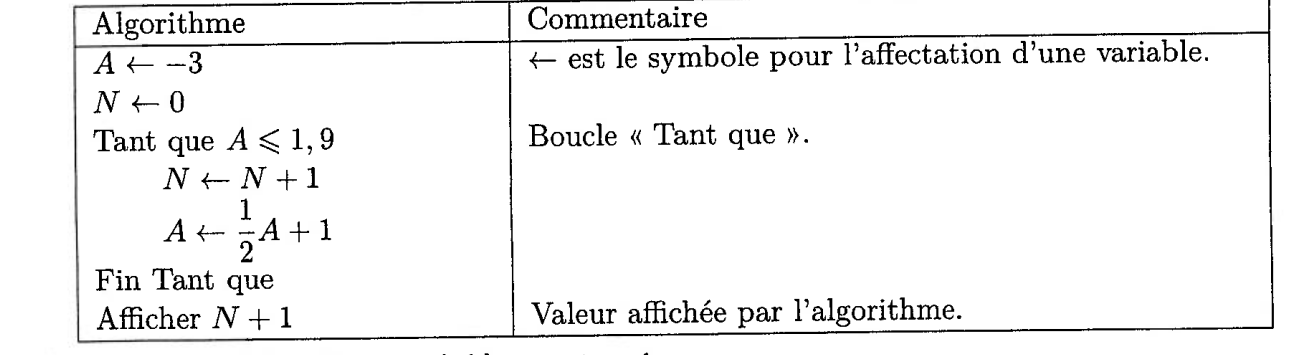
\includegraphics[scale=0.3]{vrai-faux.png}
\end{figure}

\item  On décide de lancer un dé parfaitement équilibré, dont les faces sont numérotées de $1$ à $6$, jusqu'à obtenir la face $6$. Recopier et compléter l'algorithme ci-dessous, affichant le nombre de lancers nécessaires pour obtenir la face $6$ dans cette expérience aléatoire.  \begin{figure}[H]
\centering 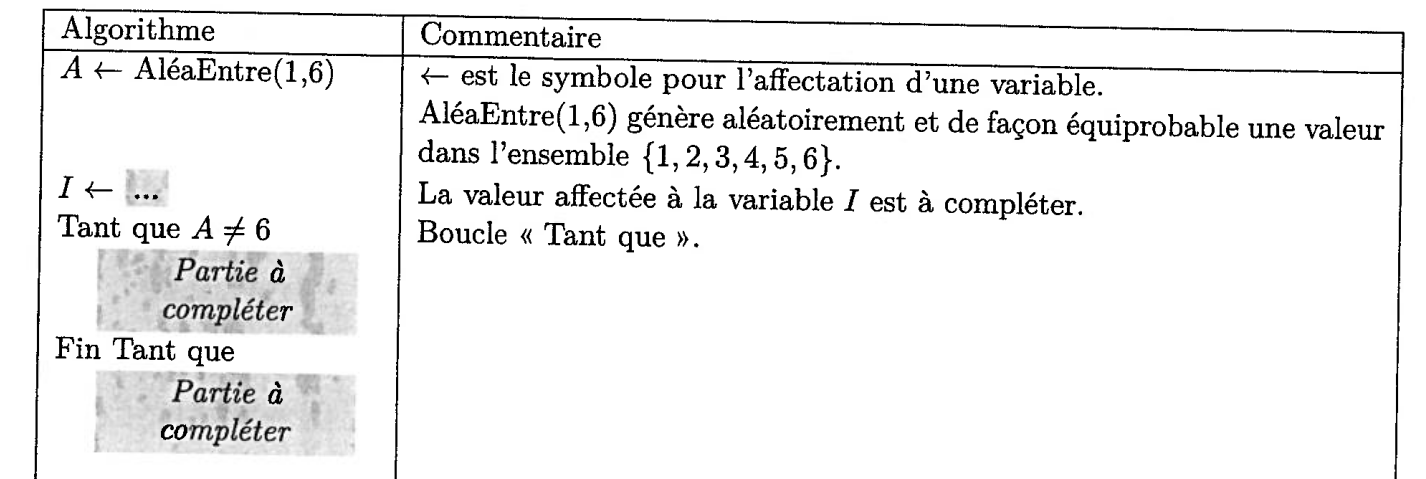
\includegraphics[scale=0.3]{de.png}

\end{figure}

\end{enumerate}
\end{ex}


 


\end{document}
